\documentclass[fullpage]{article}
\usepackage{graphicx}
\usepackage{enumerate}

\title{\vspace*{-2cm}\bf Assignment 3 - COMP 3400}
\author{Khalil Van Alphen\\
Student Number: 100863992\\
Email: \  khalil.va@gmail.com}
\date{}
\begin{document}
\maketitle
\pagestyle{plain}
\thispagestyle{empty}

\noindent 1. \ A binary adder is shown in Figure 1. The adder, on test inputs may be showing
unintended  results. Actually, the input values are:
\ $A=0, \ B=1,\ C=0$; and the output values are: $D=0 \ E=1$.\\
\\
(a) Outside Prover9 (using formulas written with Latex), construct a weak-failure model of the circuit using {\bf PROPOSITIONAL LOGIC}.
\ {\bf Explain each formula and its role in the model. Start by listing the propositional variables and their intended meanings.}\\

\noindent {\bf Solution:} \ We will use the propositional variables as listed below:
\begin{itemize}
\item[$A$:]~ {\em Input A has power.}
\item[$B$:]~ {\em Input B has power.}
\item[$C$:]~ {\em Input C has power.}
\item[$D$:]~ {\em Output D has power.}
\item[$E$:]~ {\em Output E has power.}
\item[$X$:]~ {\em Wire X has power.}
\item[$Y$:]~ {\em Wire Y has power.}
\item[$Z$:]~ {\em Wire Z has power.}
\end{itemize}
From the diagram of the circuit, we are able to construct the following propositional formulas:
\begin{itemize}
\item[$\varphi_0$:]~ ${A \oplus B \rightarrow X}$.
 Meaning: ``X has power if only one of A or B has power."
 \item[$\varphi_1$:]~ ${A \wedge B \rightarrow Y}$.
 Meaning: ``Y has power if A and B have power."
 \item[$\varphi_2$:]~ ${X \wedge C \rightarrow Z}$.
 Meaning: ``Z has power if X and C have power."
\item[$\varphi_3$:]~ ${X \oplus C \rightarrow D}$.
 Meaning: ``D has power if only one of X or C has power."
\item[$\varphi_4$:]~ ${Z \vee Y \rightarrow E}$.
 Meaning: ``E has power if Z or Y have power."
\end{itemize}


(b) You want to obtain minimal {\em conflicts}, that is, sets of components that cannot be all simultaneously working well  at the light of the observation. \ (Minimality means in this case that no proper subset of a conflict is a conflict.) Before going into Prover9, explain your methodology based on automated reasoning \`a la Prover9 for obtaining: (a) conflicts, (b) minimal ones (how can you be sure?), and (c) more than one with the same general specification.\\
\noindent {\bf Solution:}

Conflicts are easily determined when the problem is modeled as a satisfiability problem in conjunctive normal form. Each of the given formulas is a clause. Using equivalence, it is simply a matter of transforming more complex operators into NOT, AND and OR, then arranging the variables to the clausal form. Since we know the values of the power at each location, we can substitute 1 for power, and 0 for no power.

\begin{itemize}
\item[$\varphi_0$:]~ ${0 \oplus 1 \rightarrow X}$.
 \item[$\varphi_1$:]~ ${1 \wedge 1 \rightarrow Y}$.
 \item[$\varphi_2$:]~ ${X \wedge 0 \rightarrow Z}$.
\item[$\varphi_3$:]~ ${X \oplus 0 \rightarrow 0}$.
\item[$\varphi_4$:]~ ${Z \vee Y \rightarrow 1}$.
\end{itemize}

We can then look at these for conflicts by reduction.

\begin{itemize}
\item[$\varphi_0$:]~ ${X = 1}$.
 \item[$\varphi_1$:]~ ${Y = 1}$.
 \item[$\varphi_2$:]~ ${Z = 0}$. (Simplification)
\item[$\varphi_3$:]~ ${1 \oplus 0 \rightarrow 0}$. (Conflict)
\item[$\varphi_4$:]~ ${0 \vee 1\rightarrow 1}$.
\end{itemize}

(c) Use Prover9 to obtain all possible minimal conflicts. Show the main ingredients of the input file, with an
explanation. Do the same with the output file, interpreting and explaining the results.\\
\noindent {\bf Solution:}\\
INPUT:
{\small
\begin{verbatim}
	formulas(assumptions).

X <-> (-A & B) | (A & -B).
D <->(-X & C) | (X & -C).
E <-> Z | Y.
Y <-> A & B.
Z <-> X & C.

end_of_list.

formulas(goals).

B & -A & C & -D & E.

end_of_list.

 \end{verbatim}
}
OUTPUT:
{\small
\begin{verbatim}
formulas(sos).
-X | -A | -B.  [clausify(1)].
-X | B | A.  [clausify(1)].
X | A | -B.  [clausify(1)].
X | -A | B.  [clausify(1)].
-D | -X | -C.  [clausify(2)].
-D | C | X.  [clausify(2)].
D | X | -C.  [clausify(2)].
D | -X | C.  [clausify(2)].
-E | Z | Y.  [clausify(3)].
E | -Z.  [clausify(3)].
E | -Y.  [clausify(3)].
-Y | A.  [clausify(4)].
-Y | B.  [clausify(4)].
Y | -A | -B.  [clausify(4)].
-Z | X.  [clausify(5)].
-Z | C.  [clausify(5)].
Z | -X | -C.  [clausify(5)].
B.  [assumption].
-A.  [assumption].
C.  [assumption].
-D.  [assumption].
E.  [assumption].
end_of_list.
 \end{verbatim}
}
The key thing to understand is the nature of the conflict in the circuit. The reduction done by Prover9  exposes the contradiction given the set of values in this system.\\
 
\noindent 2. \ (a) Produce a knowledge base (program) in {\bf PROPOSITIONAL PROLOG} capturing the following information as closely as possible as stated here: {\em If Tweety is a bird and it is not an abnormal bird, then it flies. \
A bird is abnormal exactly when it is an ostrich, a penguin, or not an abnormal wooden bird. A wooden bird is abnormal exactly when operated under remote control. Tweety is a bird, it is  not
an ostrich nor a penguin nor a remote controlled wooden bird.}  \ {\bf All this has to be provided as a set of clauses (rules) outside Prolog, using formulas written in Latex. Start by listing the propositional variables and their intended meanings.} Notice that the two forms of abnormality mentioned here may be different, one is if birds, the other is for wooden birds.\\
\begin{itemize}
\item[$a$:]~ {\em Tweety is a bird}
\item[$b$:]~ {\em Tweety flies}
\item[$c$:]~ {\em A bird is abnormal}
\item[$d$:]~ {\em A bird is an ostrich}
\item[$e$:]~ {\em A bird is a penguin}
\item[$f$:]~ {\em A bird is an abnormal wooden bird}
\item[$g$:]~ {\em A bird is operated by remote control}
\item[$h$:]~ {\em A bird is wooden}
\end{itemize}
From this we are able to deduce a the following propositional formulas:
\begin{itemize}
\item[$\varphi_0$:]~ ${(a \wedge \neg c) \rightarrow b}$.

 Meaning: ``If Tweety is a bird and it is not an abnormal bird, then Tweety flies."
\item[$\varphi_1$:]~ ${(d \lor e \lor \neg f) \rightarrow c}$

     Meaning: ``If a bird is an ostrich, a penguin or not an abnormal wooden bird, it is abnormal."
\item[$\varphi_2$:]~ ${(h \wedge g) \rightarrow f}$

 Meaning: ``If a bird is wooden and remote controlled, it is an abnormal wooden bird."
\item[$\varphi_3$:]~ ${a}$

 Meaning: ``Tweety is a bird."
\item[$\varphi_4$:]~ ${\neg d}$

 Meaning: ``Tweety is not an ostrich."
\item[$\varphi_5$:]~ ${\neg e}$

 Meaning: ``Tweety is not a penguin."
\item[$\varphi_6$:]~ ${\neg h}$

 Meaning: ``Tweety is not wooden."
\item[$\varphi_7$:]~ ${\neg g}$

 Meaning: ``Tweety is not remote controlled."
\end{itemize}

We are able to construct the formula:
${a \wedge \neg(d \vee e \vee \neg (h \wedge g))) \rightarrow b}$\\

\noindent (b) Show by means of a refutation tree developed \'a la Prolog that  {\em Tweety flies} \ (as we did in class).\\

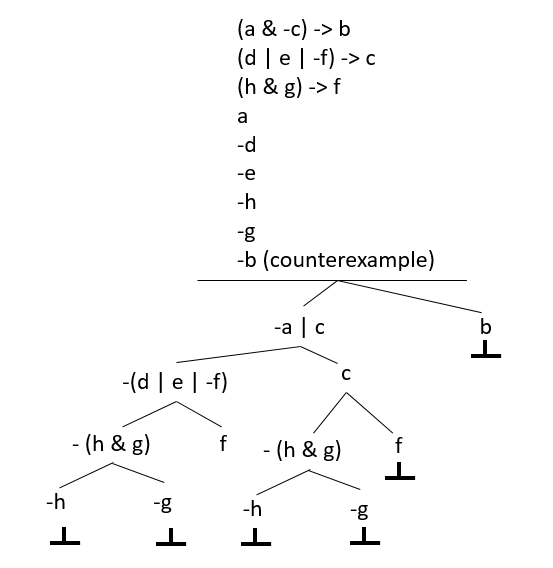
\includegraphics[scale=0.4]{cp}

(c) Now use SWI Prolog to prove that {\em Tweety flies}. Explain your approach and what Prolog shows through its run. Attach a file showing the input file, and the whole run (interaction, trace) with Prolog.  \\

\newpage
\section*{Appendix: Input/Output Files}
1.INPUT:

 {\footnotesize \begin{verbatim}
set(ignore_option_dependencies). % GUI handles dependencies

if(Prover9). % Options for Prover9
  assign(max_seconds, 60).
end_if.

if(Mace4).   % Options for Mace4
  assign(max_seconds, 60).
end_if.

formulas(assumptions).

X <-> (-A & B) | (A & -B).
D <->(-X & C) | (X & -C).
E <-> Z | Y.
Y <-> A & B.
Z <-> X & C.

end_of_list.

formulas(goals).

B & -A & C & -D & E.

end_of_list.


\end{verbatim} }

1.OUTPUT:

 {\footnotesize \begin{verbatim}
============================== Prover9 ===============================
Prover9 (32) version Dec-2007, Dec 2007.
Process 57436 was started by Khalil on Khalil-PC,
Tue Mar  7 04:11:52 2017
The command was "/cygdrive/c/Program Files (x86)/Prover9-Mace4/bin-win32/prover9".
============================== end of head ===========================

============================== INPUT =================================
assign(report_stderr,2).
set(ignore_option_dependencies).
if(Prover9).
% Conditional input included.
assign(max_seconds,60).
end_if.
if(Mace4).
% Conditional input omitted.
end_if.

formulas(assumptions).
X <-> -A & B | A & -B.
D <-> -X & C | X & -C.
E <-> Z | Y.
Y <-> A & B.
Z <-> X & C.
end_of_list.

formulas(goals).
B & -A & C & -D & E.
end_of_list.

============================== end of input ==========================

% Enabling option dependencies (ignore applies only on input).

============================== PROCESS NON-CLAUSAL FORMULAS ==========

% Formulas that are not ordinary clauses:
1 X <-> -A & B | A & -B # label(non_clause).  [assumption].
2 D <-> -X & C | X & -C # label(non_clause).  [assumption].
3 E <-> Z | Y # label(non_clause).  [assumption].
4 Y <-> A & B # label(non_clause).  [assumption].
5 Z <-> X & C # label(non_clause).  [assumption].
6 B & -A & C & -D & E # label(non_clause) # label(goal).  [goal].

============================== end of process non-clausal formulas ===

============================== PROCESS INITIAL CLAUSES ===============

% Clauses before input processing:

formulas(usable).
end_of_list.

formulas(sos).
-X | -A | -B.  [clausify(1)].
-X | B | A.  [clausify(1)].
X | A | -B.  [clausify(1)].
X | -A | B.  [clausify(1)].
-D | -X | -C.  [clausify(2)].
-D | C | X.  [clausify(2)].
D | X | -C.  [clausify(2)].
D | -X | C.  [clausify(2)].
-E | Z | Y.  [clausify(3)].
E | -Z.  [clausify(3)].
E | -Y.  [clausify(3)].
-Y | A.  [clausify(4)].
-Y | B.  [clausify(4)].
Y | -A | -B.  [clausify(4)].
-Z | X.  [clausify(5)].
-Z | C.  [clausify(5)].
Z | -X | -C.  [clausify(5)].
-B | A | -C | D | -E.  [deny(6)].
end_of_list.

formulas(demodulators).
end_of_list.

============================== PREDICATE ELIMINATION =================

No predicates eliminated.

============================== end predicate elimination =============

Auto_denials:  (non-Horn, no changes).

Term ordering decisions:
Predicate symbol precedence:  predicate_order([ X, A, B, C, Y, Z, D, E ]).
Function symbol precedence:  function_order([ ]).
After inverse_order:  (no changes).
Unfolding symbols: (none).

Auto_inference settings:
  % set(binary_resolution).  % (non-Horn)
  % set(neg_ur_resolution).  % (non-Horn, less than 100 clauses)

Auto_process settings:
  % set(factor).  % (non-Horn)
  % set(unit_deletion).  % (non-Horn)

============================== end of process initial clauses ========

============================== CLAUSES FOR SEARCH ====================

% Clauses after input processing:

formulas(usable).
end_of_list.

formulas(sos).
7 -X | -A | -B.  [clausify(1)].
8 -X | B | A.  [clausify(1)].
9 X | A | -B.  [clausify(1)].
10 X | -A | B.  [clausify(1)].
11 -D | -X | -C.  [clausify(2)].
12 -D | C | X.  [clausify(2)].
13 D | X | -C.  [clausify(2)].
14 D | -X | C.  [clausify(2)].
15 -E | Z | Y.  [clausify(3)].
16 E | -Z.  [clausify(3)].
17 E | -Y.  [clausify(3)].
18 -Y | A.  [clausify(4)].
19 -Y | B.  [clausify(4)].
20 Y | -A | -B.  [clausify(4)].
21 -Z | X.  [clausify(5)].
22 -Z | C.  [clausify(5)].
23 Z | -X | -C.  [clausify(5)].
24 -B | A | -C | D | -E.  [deny(6)].
end_of_list.

formulas(demodulators).
end_of_list.

============================== end of clauses for search =============

============================== SEARCH ================================

% Starting search at 0.00 seconds.

given #1 (I,wt=3): 7 -X | -A | -B.  [clausify(1)].

given #2 (I,wt=3): 8 -X | B | A.  [clausify(1)].

given #3 (I,wt=3): 9 X | A | -B.  [clausify(1)].

given #4 (I,wt=3): 10 X | -A | B.  [clausify(1)].

given #5 (I,wt=3): 11 -D | -X | -C.  [clausify(2)].

given #6 (I,wt=3): 12 -D | C | X.  [clausify(2)].

given #7 (I,wt=3): 13 D | X | -C.  [clausify(2)].

given #8 (I,wt=3): 14 D | -X | C.  [clausify(2)].

given #9 (I,wt=3): 15 -E | Z | Y.  [clausify(3)].

given #10 (I,wt=2): 16 E | -Z.  [clausify(3)].

given #11 (I,wt=2): 17 E | -Y.  [clausify(3)].

given #12 (I,wt=2): 18 -Y | A.  [clausify(4)].

given #13 (I,wt=2): 19 -Y | B.  [clausify(4)].

given #14 (I,wt=3): 20 Y | -A | -B.  [clausify(4)].

given #15 (I,wt=2): 21 -Z | X.  [clausify(5)].

given #16 (I,wt=2): 22 -Z | C.  [clausify(5)].

given #17 (I,wt=3): 23 Z | -X | -C.  [clausify(5)].

given #18 (I,wt=5): 24 -B | A | -C | D | -E.  [deny(6)].

============================== STATISTICS ============================

Given=18. Generated=18. Kept=18. proofs=0.
Usable=18. Sos=0. Demods=0. Limbo=0, Disabled=18. Hints=0.
Weight_deleted=0. Literals_deleted=0.
Forward_subsumed=0. Back_subsumed=0.
Sos_limit_deleted=0. Sos_displaced=0. Sos_removed=0.
New_demodulators=0 (0 lex), Back_demodulated=0. Back_unit_deleted=0.
Demod_attempts=0. Demod_rewrites=0.
Res_instance_prunes=0. Para_instance_prunes=0. Basic_paramod_prunes=0.
Nonunit_fsub_feature_tests=0. Nonunit_bsub_feature_tests=18.
Megabytes=0.03.
User_CPU=0.00, System_CPU=0.01, Wall_clock=0.

============================== end of statistics =====================

============================== end of search =========================

SEARCH FAILED

\end{verbatim} }

\end{document} 
